\documentclass[journal]{IEEEtran}
\usepackage{lipsum}
\usepackage{researchPaper}

%Useful for [1]-[3]
%\usepackage{cite}

%Algorithms
%\usepackage{algorithm}
%\usepackage{algorithmic}

%\usepackage{listings}

%Math Packages
%\usepackage{amsmath}
%\usepackage{amssymb}


%\usepackage{commath} %derivative, norm etc.
%\usepackage{physics}
%\usepackage{bm} %bold

%Figure packages
%\usepackage{float}
%\usepackage{graphicx}
%\usepackage[justification=centering]{caption}
%\usepackage{tikz}
%\usetikzlibrary{matrix}

\begin{document}

\title{Sample Latex Showing Various Features for Research Papers}

\author{Christopher~Fadden \\
        School~of~Electrical~Engineering~and~Computer~Science \\
        Pennsylvannia~State~University \\
        State College,~PA,~USA}

% make the title area
\maketitle

\begin{abstract}
  \lipsum[1]
\end{abstract}

\begin{IEEEkeywords}
  Greek Equations, Matrices, Tables, Figures, Source Code, Theorems
\end{IEEEkeywords}

\section{Introduction} \label{sec: intro}

\IEEEPARstart{M}{Aspell's} Equations, derived in 1865, give the governing 
equations of electrodynamics \cite{Maxwell}.  These equations can only be solved
analytically for a few simple cases and structures.  Approximations to complex 
structures must be made in order to solve these problems with a pencil and 
paper.  However, when a high degree of accuracy is required, numerical techniques 
must be used.  Different numerical techniques are used depending on the problem.
The Finite Difference Time Domain (FDTD) takes the full three dimensional 
Maxwell’s Equations, and approximates the derivatives using finite differences 
\cite{Yee}.  With a coarse enough grid, the FDTD gives results that closely 
agree with experimental measurements.  However, in order to implement the 
coarseness of the grid, verbose computing languages such as FORTRAN or C++ must
be used.  This leads to a program on the order of 1,000 lines of code, which is 
difficult to maintain and prone to error.  However, the accuracy and scope of 
this technique means it is used to measure fields related to antennas, waveguides,
and other structures of interest to electrical engineers. 

The Scatter Matrix Method takes a different approach than the FDTD.  Rather than
expressing Maxwell’s Equations using finite differences, the Scatter Matrix 
Method rewrites the equations in a matrix wave equation form.  The structures 
modeled   are assumed to be homogeneous in two directions, simplifying the 
problem from 3D to 1D.  By simplifying the problem this way, the operators 
involved are 2x2 matrices.  The simplifications made, 
and the fact that the Scatter Matrix Method is inherently a frequency-domain 
method, mean it is much simpler to implement using a computer.  High-level 
computing languages, such as MATLAB or Python can implement this technique on 
the order of 300 lines of code.  The abstractions allowed by these languages, as
well as the shortness of the code, makes it very easy to implement, and because 
there are fewer computations, it runs in a reasonable time frame.  This technique
is very attractive for members of the optical electronics community, where the 
assumptions described are often valid.  However, the assumptions made do not apply 
to structures used by members of the radio frequency (RF) or microwave community, 
meaning that this technique is only a first approximation to these relatively 
lower frequency disciplines.  For high accuracy in RF or microwave circuits, 
the FDTD is the better option. 



\section{Citations} \label{sec:cites}
  \subsection{Books}
  This is a section on citations.  The first citation is a series of books, and
  shows how the edition doesn't matter 
  \cite{balanis_advanced_2012,poor_introduction_1998,mallat_wavelet_1998}.  
  That also used three references \cite{hastie_statistical_2015}.

  \subsection{Articles}
    This references a normal journal \cite{berger_adaptive_1984}.  Now we want
    to cite the normal IEEE journals \cite{gao_method_2004,manikas_array_2013}.
    And finally a conference paper \cite{bond_microwave_2002}.

\section{Equations} \label{sec:Equations} 
  This demonstrates various equations.
  
  Numbered vs unnumbered equations:

  \begin{equation}
    \vec{w} = a \vec{x} + \vec{y}   %Vectors
  \end{equation}
  
  \begin{equation*}
    \begin{aligned}
      x - y \approx z \\            %approx
      x + y \ge z \\                %greater than or equal to 
      x + w \le z \\                %less than or equal to
      x \in \mathbb{R}^n \\         %set notation
      y \to x - z^{\dagger} \\      %Hermitian dagger
    \end{aligned}
  \end{equation*}
  
  Optimization algorithms

  \begin{equation}
    \begin{aligned}
      & \underset{\bm{x}}{\text{minimize}}
      & & \bm{x}^T A \bm{x} \\
      & \text{subject to}
      & & \norm{\bm{x}} < 1 \\          %norm and bold operations
    \label{eq:EQlabel}
    \end{aligned}
  \end{equation}
 
  Equations can be referenced (\ref{eq:EQlabel}).

 \begin{equation*}
  \begin{aligned}
      & & \od[4]{f}{x} = \pd[4]{f}{x} \\              %ODE / PDE
      & & \frac{x - 4}{5} = \md{f}{5}{x}{2}{y}{2} \\  %mixed partials
      & & A = \iiint \mu \vec{J} dV \\                %integrals
      & & x = \sum_{i=1}^N a_ib_i \\                  %sums
  \end{aligned}
 \end{equation*}

  \begin{equation}
    \bra{\Psi}\ket{\Psi} = \begin{bmatrix}            %Bra Ket and matrix
                              1 & 0 & 0 \\
                              0 & 1 & 0 \\
                              0 & 0 & 1 \\
                            \end{bmatrix}
  \end{equation}
  
  And here's some polynomial magic
  \begin{equation}
    \polylongdiv{X^3 + X^2 - 1}{X-1}                  %Polynomial long division magic
  \end{equation}

  \begin{equation}
    \polyset{vars=Y}
    \polyfactorize{2Y^3 + Y^2 - 7Y + 3}               %Magic factoring polynomials
  \end{equation}

  


  %including Pictures
  %creating own via tikz

  \begin{figure}[H] 
    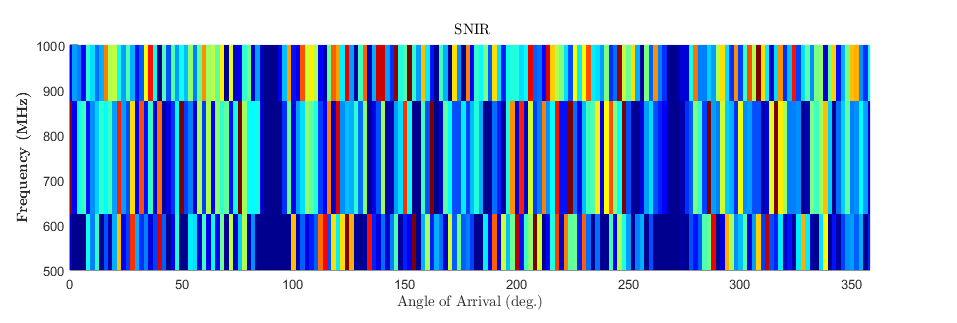
\includegraphics[width=0.5\textwidth]{./fig/pic/pic.png}
    \caption{A sample figure}
\end{figure}

  \begin{figure}[H]
\begin{tikzpicture}
  \matrix (m) [matrix of math nodes, row sep=3em,
    column sep=3em]{
    & f^\ast E_V& & \vphantom{f^\ast}E_V \\
    f^\ast E & & \vphantom{f^\ast}E & \\
    & U & & V \\
    M & & N & \\};
  \path[-stealth]
    (m-1-2) edge (m-1-4) edge (m-2-1)
            edge [densely dotted] (m-3-2)
    (m-1-4) edge (m-3-4) edge (m-2-3)
    (m-2-1) edge [-,line width=6pt,draw=white] (m-2-3)
            edge (m-2-3) edge (m-4-1)
    (m-3-2) edge [densely dotted] (m-3-4)
            edge [densely dotted] (m-4-1)
    (m-4-1) edge (m-4-3)
    (m-3-4) edge (m-4-3)
    (m-2-3) edge [-,line width=6pt,draw=white] (m-4-3)
            edge (m-4-3);
\end{tikzpicture}
\label{fig:tikzExample}
\caption{This is an example of TikZ}
\end{figure}


  %Tables (w/ R)
  % latex table generated in R 3.3.2 by xtable 1.8-2 package
% Thu Jan  5 17:49:56 2017
\begin{table}[ht]
\centering
\caption{Interferers at 60, 200 and 340 deg. with Dipole Array} 
\label{tab:feko60_200_340}
\begin{tabular}{rlllll}
  \hline
 & Time (s) & Low SINR (dB) & Mid SINR (dB) & High SINR (dB) & BW (deg) \\ 
  \hline
MVDR & -- & 12.63 & 14.76 & 15.57 & -- \\ 
  CMA-ES & 2380 & 7.52 & 3.96 & 6.66 & -- \\ 
  Genetic Algorithm & 1900 & 2.30 & 1.76 & 6.22 & -- \\ 
  Conjugate Gradient & 0.270 & 0.17 & 0.71 & 1.03 & -- \\ 
  GSC & 0.232 & 0.06 & 0.45 & 1.85 & -- \\ 
  DD3 & 0.295 & 8.86 & 2.40 & 5.90 & -- \\ 
   \hline
\end{tabular}
\end{table}

  
  %Theorems
     
  %Algorithms
  \begin{algorithm}
    \caption{Conjugate Gradient Method}
      \label{alg:cg}
      \begin{algorithmic}
        \STATE $\vec{r}_0 \rightarrow \vec{a}(\phi,\theta) - R_{yy}\vec{w}$
        \STATE $\vec{p}_0 \rightarrow \vec{r}_0$
        \WHILE{$|\vec{r_i}| > tolerance$}
          \STATE $a_i \rightarrow \frac{\vec{r}_i^T \vec{r}_i}{\vec{p}_i^T R_{yy}\vec{p}_i}$
          \STATE $\vec{w}_{i+1} \rightarrow \vec{w} + a_i \vec{p}_i$
          \STATE $\vec{r}_{i+1} \rightarrow \vec{r}_i - a_i R_{yy}\vec{p}_i$
          \STATE $b_i \rightarrow \frac{\vec{r}_{i+1}^T\vec{r}_{i+1}}{\vec{r}_i^T\vec{r}_i}$
          \STATE $\vec{p}_{i+1} \rightarrow \vec{r}_{i+1} + b_i \vec{p}$
        \ENDWHILE
      \end{algorithmic}
    \end{algorithm}
  
  %Inputting code from elsewhere 
  \lstinputlisting[language=R,basicstyle=\small]{./table/tableMaker.r}

\bibliographystyle{IEEEtran}
\bibliography{Test.bib}

\end{document}
